% !TEX root = ../main.tex

\chapter[О естественности байесовского мышления]{О покере, Баесовском мышлении и его естественности}


\epigraph{Если вы сомневаетесь в практической применимости теоремы байеса, то, возможно, вы никогда не видели, как играют в покер.}{\textit{Нейт Сильвер. Сигнал и шум }}

В этой главе мы поговорим о философии, которая лежит за байесовским подходом и попробуем понять в чём выражается его естественность. Делать мы это будем практически без формул. 


\section{Немного истории} 

Томас Байес был английским священником, родившимся толи в 1701, толи в 1702 году. О жизни его известно довольно мало, хотя он подарил своё имя целому направлению в статистике и, возможно, самой знаменитой её теореме.  Неясно даже как выглядел Байес на самом деле, его портрет, который часто приводят в энциклопедях, может принадлежать другому человеку.

Родители Томаса, и он сам,  принадлежали к церкви нонкомформистов, а не англиканской. В связи с этим ему был закрыт путь в учебные заведения типа Оксфорда и Кембриджа. В 1719 году он поступил в Эдинбургский университет, который впоследствии успешно окончил.

\begin{wrapfigure}{r}{0.3\textwidth}
	\centering 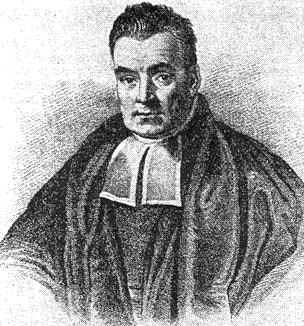
\includegraphics[width=0.8\linewidth]{images/bayes.png}
	\caption{Портрет Томаса Байеса (но это неточно)}
\end{wrapfigure}

За свою жизнь Байес написал две работы: одну богословскую, трактат <<Божественная доброта>>, вторую математическую, <<Очерки к решению проблемы доктрины шансов>>. Тем не менее, это не помешало ему стать членом Королевского научного общества. Байес был весьма известным среди современных ему английских учёных человеком. Внутри общества он обычно выполнял роль внутреннего критика или был посредником в ходе интеллектуальных дебатов.

Математическая работа Байеса увидела свет только после его смерти. В 1763 году она была представлена вниманию Королевского общества его другом, Ричардом Прайсом, который обновил и дополнил работу. Сам того не подозревая Байес стал центром новой религии. Его теорема стала настолько популярной, что её даже показали в телешоу <<Теория Большого взрыва>>.

\begin{wrapfigure}{l}{0.3\textwidth}
	\centering 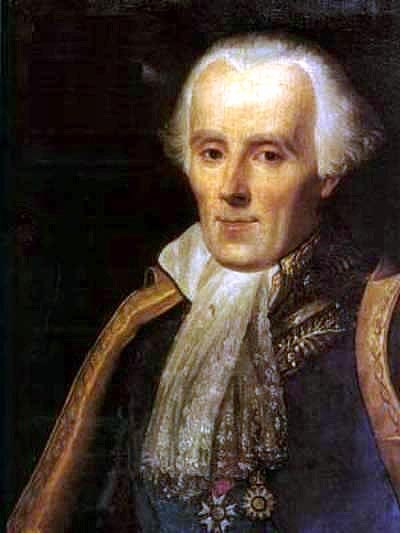
\includegraphics[width=0.8\linewidth]{images/laplas.jpg}
	\caption{Портрет Пьера-Симона Лапласа (это почти наверное)}
\end{wrapfigure}

В работе Байеса впервые вводилось достаточно строгое определение понятия условной вероятности и решалась типичная задача байесовского вывода. Давайте представим себе человека, попадающего в наш мир и впервые видящего восход солнца. Поначалу он не знает, насколько обычным является это явление, и о том взойдёт ли солнце завтра ему остаётся только гадать. Бедняга вообще ничего не знает о солнце! Он вынужден рассматривать два одинаково вероятных варианта и сказать, что солнце снова взойдёт с вероятностью $\frac{1}{2}$.

Каждый новый день, новоиспечённый житель Земли наблюдает за тем, как восходит солнце. Это укрепляет его уверенность в том, что так будет происходить и дальше.  Каждый день вероятность пересчитывается по формуле $\frac{n+1}{n+2}$ и становится всё ближе к единице. Однако с единицей эта вероятность не сравняется, потому что полной уверенности в восходе солнца не будет никогда.

Теорема Байеса --- это простое правило обновления уровня доверия к гипотезе при получении новых доказательств: если свидетельство совпадет с гипотезой, её вероятность возрастает, если нет, то убывает.   Философия Байеса даёт нам способ изучать Вселенную. Мы учимся новым представлениям о ней с помощью аппроксимаций, оказываясь ближе и ближе к истине по мере того, как мы собираем всё больше свидетельств.

\begin{wrapfigure}{r}{0.3\textwidth}
	\centering 
\includegraphics[width=0.8\linewidth]{images/demon.jpg}
	\caption{Портрет Демона Лапласа (но это неточно)}
\end{wrapfigure} 

Спустя какое-то время, один из отцов-основателей теории вероятностей, Пьер-Симон Лаплас сформулировал теорему Байеса в том виде, в котором она дошла до нас.  Лалпас был детерменистом. Он считал, что мы могли бы идеально спрогнозировать нашу Вселенную, если бы знали точное положение каждой частицы и могли бы быстро расчитать как они будут двигаться.   Существо, которое могло бы произвести такие вычисление было названо демоном Лапласа. Лаплас понимал, что между совершенностью природы и несовершенством человеческого познания существует огромный разрыв, и рассматривал неопределённость как результат этого разрыва.  В мире Лапласа случайность --- это результат нашего невежества, а вероятность --- это способ это невежество измерить. Вероятность --- субъективна. Отсюда вытекает основное философское различие между байесовским подходом и частотном подходом, об отце которого мы поговорим ровно через одну строку.

Английский статистик и генетик Рональд Эймлер Фишер родился в 1890 году и, несмотря на разницу в возрасте (120 лет это тебе не шутки), стал одним из основных интеллектуальных противников Томаса Байеса. Фишер более, чем кто бы то ни было другой, ответственен за тот статистический аппарат, которым мы сегодня пользуемся. Именно он обосновал оптимальность метода максимального правдоподобия и разработал методологию для проверки статистических гипотез. Впоследствии в честь Фишера было названо целое семейство распределений. 

Именно Фишер впервые использовал термин <<байесовский>> в опубликованной статье. Он утверждал, что теория Байеса должна быть полностью отвергнута. 
\begin{wrapfigure}{l}{0.3\textwidth}
	\centering 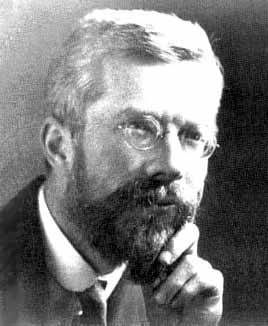
\includegraphics[width=0.8\linewidth]{images/Fischer.jpg}
	\caption{Портрет Рональда Фишера (это почти наверное)}
\end{wrapfigure} 
Частотный подход говорит, что наука не может рассматривать вероятность, как нечто субъективное. Можно оценивать вероятности только тех событий, которые происходят более одного раза, и вопросы вроде << Какова вероятность того, что на ближайших выборах победит политик номер $N$?>> не имеют ответа, потому что ещё не было таких выборов. С точки зрения частотного подхода вероятность должна быть объективной.

Фишер и его современники решили освободить мир от любого возможного негативного влияния субъективных предубеждений и искажений и разработали набор статистических методов, которые люди применяют и сегодня.

Итак, между байесовским и частотным подходом есть всего одно существенное отличие, из которого вытекают все остальные.

\begin{itemize}
\item С точки зрения байесовцев случайность субъективна. Окружающий нас мир на самом деле детерминирован, а неопределённость трактуется как часть факторов, которая нам неизвестна. В связи с этим любая неизвестная величина может интерпретироваться как случайная.

\item С точки зрения частотников случайность объективна, и мы не можем принципиально предсказать значение такой величины. Неопределённость, в свою очередь, это нечто присущее эксперименту, а не нашей способности познавать мир.
\end{itemize}

На этом моменте давайте на секундочку задумаемся о том какие случайности окружают нас в жизни. На самом деле это зависит от нашей работы. Например, если вы работаете крупье в казино, вы каждый день встречаетесь с субъективной случайностью. При желании и технической оснащённости, можно попытаться рассчитать с какой именно скоростью шарик падает на рулетку, скорректировать его падение на то как именно рулетка крутится, учесть ещё кучу разных факторов вроде скорости ветра и момента вращения, и у нас идеально получится предсказать куда именно упадёт шарик. Тем не менее, мы это не делаем, потому что у нас нет таких мощных вычислительных средств. В этом случае вероятность описывает наше невежество. Точно также неслучайно то время, через которое автобус приедет на остановку. У нас нет никакой информации что произошло с автобусом  на прошлой остановке и сколько он будет добираться до нашей. Во время его движения может столько всего произойти, и из-за того, что всего этого невозможно учесть (хотя ничего не мешает нам попробовать), мы говорим, что время его приезда случайно.

Здесь проницательный читатель может подумать, что объективной случайности в природе просто-напросто не существует, однако это не так. Объективная случайность наблюдается в квантовой физике (по крайней мере на нашем современном уровне её понимания), она вшита в наше естество на атомном уровне. 

Более того, если существует свобода воли (а это не факт), вряд ли получится предсказать что именно взбредёт человеку сделать в следующую секунду, даже обладая самыми совершенными измерительными приборами. Можно рискнуть сказать, что поведению людей свойственна объективная неопределённость\footnote{Возможно, наше будущее предопределено, но человек не может этого осознать, и у него возникает ощущение, что он на что-то влияет. В таком случае свобода воли порождается субъективным незнанием, а не объективной неопределённостью. В фильме Прибытие как раз обыгрывается то, что у нас нет органа, который чувствовал бы будущее и из-за этого эволюционного невежества возникает иллюзия свободы воли.}.

На почве этой глубокой философской разницы между двумя течениями возникает нешуточный холивар с большим количеством лулзов. Именно в этот холивар нам предстоит более глубоко погрузиться в течение следующей главы.

Но сперва нам хотелось бы, чтобы вы немного лучше прочувствовали прелести байесовского мышления и убедились в его естественности. Для этого мы приводим здесь небольшой фрагмент из книги байесовца, прогнозиста и заядлого игрока в покер Нейта Сильвера <<Сигнал и шум>> \cite{silver2012signal}.

\section{О том как люди играют в покер}

Предположим, вы играете партию в безлимитный техасский холдем\footnote{Возможно, тем, кто никогда не играл в безлимитный техасский холдем, стоит изучить \href{https://ru.wikipedia.org/wiki/Техасский_холдем}{правила этой игры.} Но мы на этом не настаиваем. } со ставками $5$ и $10$ долл. в <<Белладжио>>. Первые несколько игроков сбросили свои карты, а у вас на руках имеется вполне достойная комбинация --- пара восьмёрок ($8$\clubsuit $8$\spadesuit). Поэтому вы повышаете ставку до $25$ долл., и на неё отвечает всего один игрок, $60$-летний мужчина, которого мы будем называть Юрист.

Это довольно приятный человек. В промежутках между партиями он охотно болтает, но после раздачи смолкает. О себе он рассказал, что работает партнёром в юридической компании на Восточном побережье, занимающейся вопросами интеллектуальной собственности. Его вполне можно представить в рубашке-поло, периодически отправляющим своему другу сообщения о том, за сколько ударов ему удалось пройти дистанцию в игре в гольф. Перед тем как переключиться на кофе во время игры, он выпил один бокал пива. Судя по всему, его совершенно не пугают ставки, по которым идёт игра.

Когда Юрист только сел с нами за стол, у нас было два совершенно различных предположения о том, что он собой представляет. Первое состояло в том, что он будет немного выпендриваться во время игры, делая необоснованные шаги и блефуя, а второе --- в том, что он будет использовать строгий <<книжный>> подход. Наши последующие наблюдения подтвердили правильность второй гипотезы. Юрист создавал впечатление довольно посредственного игрока, избегавшего катастрофических ошибок, но не проявляющего особого мастерства. Вне всякого сомнения, он --- не худший из игроков, однако вряд ли может стать победителем в долгосрочной перспективе. Тем не менее мы ещё не играли против него достаточно долго и не уверены ни в одной из своих гипотез до конца.

Итак, что же мы знаем о картах Юриста в настоящий момент? Единственное, в чём не приходится сомневаться, так это в том, что у него нет комбинации с картами $8$\clubsuit  или $8$\spadesuit, поскольку эти карты --- наши. К сожалению, это снижает количество начальных комбинаций всего лишь с $1326$ до $1225$, причем каждая из них имеет одинаковые шансы быть у него на руках.

Тем временем мы получили от Юриста дополнительную информацию --- он решил ответить на нашу ставку. Это значит, что его комбинация должна быть как минимум достойной --- основная часть игроков, включая Юриста, сбрасывают карты в большинстве случаев, а не поднимают ставки перед флопом. И это значит также, что у него вряд ли очень сильная комбинация типа пары тузов, поскольку он просто ответил на нашу ставку, а не поднял её ещё выше, хотя нельзя исключать, что он хитрит.

Мы можем приступить к формированию вероятностной байесовской оценки карт, которые могут быть на руках у Юриста. Из прошлого опыта игры с похожими на него людьми мы знаем, что у него на руках вполне могут оказаться пары типа  $9\vardiamond$  $9$\spadesuit. Также комбинация может включать в себя туза, особенно если обе карты относятся к одной масти (например, $A\varheart$  $5\varheart$), что даёт ему возможность собрать флэш. Также у него на руках могут быть так называемые одномастные коннекторы --- карты типа $6$\spadesuit.  $5$\spadesuit., принадлежащие к одной масти, идущие по номиналу одна за другой и позволяющие собрать флэш или стрит. И, наконец, он мог ответить вам двумя старшими картами, например $J \vardiamond$  $K$\spadesuit.

Если бы у нас было достаточно времени, мы могли бы перечислить все комбинации, которые могут быть на руках у Юриста, и привели для каждой значение вероятности от $0$ до $1$, с учётом его действий к настоящему моменту. Именно так оценивал бы его игру компьютер, способный быстро обрабатывать вероятности.

На практике игроки обычно разбивают диапазон возможных комбинаций карт на группы, в отношении которых оппонент будет предпринимать одинаковые действия. В данном случае самой опасной для нас на данный момент выступает группа комбинаций с парой, старше нашей пары восьмёрок.

К счастью, вероятность подобного развития событий мала: игроку в холдем редко удаётся получить такую пару карт с самого начала. Однако, учитывая, что Юрист ответил на нашу ставку, нам следует обновить просчитанное значение этой вероятности --- чаще всего этот игрок сбрасывает слабые карты, а следовательно, сейчас у него на руках что-то есть. Главная проблема состоит в том, что на столе должно появиться ещё пять карт, и хотя шансов на то, что они улучшат нашу пару довольно мало (нам потребуется одна из оставшихся восьмёрок), Юрист может довольно легко собрать более высокую пару, стрит или флэш.

Юрист отпивает немного кофе, пока дилер выкладывает карты флопа в центре стола. Это две трефы --- король и тройка, --- а также девятка червей,   $K$\clubsuit  $9\varheart$  $3$\clubsuit.

Эти карты не сделали нашу комбинацию лучше. Остаётся лишь надеяться, что они не улучшили и комбинацию, которая на руках у Юриста и наша пара восьмёрок всё равно останется самой сильной.

Поэтому мы делаем довольно скромную ставку, добавляя $35$ долл. в банк, составляющий уже $65$ долл. Юрист на мгновение делает паузу, а затем отвечает на нашу ставку.

Его поступок нас не удивляет, и мы приступаем к перерасчёту вероятностей его комбинации. Согласно теореме Байеса, главное --- размышлять в понятиях условных вероятностей. Например, если Юрист начал игру с комбинацией типа $J \vardiamond$  $K$\spadesuit, а теперь у него появилась пара королей, насколько вероятно, что он вновь ответит на нашу ставку? (Разумеется, с сильной парой на руках он вполне может это сделать, но не лучше ли для него было бы поднять ставку выше?) А что, если он начал игру с меньшей парой, например $ 7\varheart, 7$\spadesuit, --- насколько вероятно, что он ответит нам, а не сбросит карты? Если бы у нас было больше времени, мы могли бы изучить каждую из $1326$ комбинаций и соответствующим образом пересмотреть свои расчёты.

Наши реальные расчёты, которые мы делаем за столом, будут куда менее точными. Тем не менее мы можем с учётом действий Юриста дать определённые, причём довольно широкие, вероятностные характеристики диапазона возможных комбинаций у него на руках. Примерно в $30\%$ случаев комбинация карт Юриста собиралась с учётом флопа, и он имел пару королей или более сильную комбинацию. Это хорошие комбинации, и при отсутствии сильного внешнего давления он не стал бы их сбрасывать. Имеется также $20\%$-ная вероятность, что у него на руках пара хуже, чем короли, но лучше, чем наши восьмёрки. Эти комбинации переигрывают нашу, однако, если мы продолжим агрессивно повышать ставки, Юрист, скорее всего, их сбросит.

Имеется также $25\%$-ная вероятность, что Юрист имеет шансы собрать стрит или флэш. На данный момент его карты значительно слабее наших, однако у него есть возможность улучшить ситуацию.

И, наконец, вероятность, что у Юриста есть пара меньше нашей или нет вообще ничего, составляет $25\%$, и он продолжает делать ставки в надежде на будущий блеф. Этот вариант для нас самый предпочтительный.

Вы можете сами увидеть, насколько сложно порой принимать решения в покере. Если верны одни варианты, мы должны делать максимально агрессивные ставки. Если другие, мы должны ограничиться более осторожным подходом, а если третьи, мы должны готовиться к тому, чтобы сбросить карты.

Пока мы размышляем, принимая это отнюдь не простое решение, дилер кладёт на стол идеальную для нас карту, чем ощутимо заметно улучшает нашу жизнь. Это одна из двух восьмёрок, оставшихся в колоде, $8\vardiamond$, и в результате у нас возникает набор из трёх одинаковых карт. Единственная комбинация, при которой мы можем проиграть, возникнет, если Юрист начал игру с парой девяток или королей, получил набор из трёх одинаковых карт на флопе, а затем начал играть пассивно, чтобы заманить нас в ловушку (для этого у игроков в покер есть специальный термин <<слоуплей>>). Но нам не стоит чрезмерно осторожничать. Какова бы ни была комбинация у Юриста, наши шансы на победу составляют примерно $98\%$. Поэтому мы делаем сравнительно крупную ставку --- $100$ долл. при банке в $135$ долл.

Юрист ещё раз отвечает на нашу ставку. Если бы у него была слабая пара или не сформированная комбинация, он, скорее всего, сбросил бы карты. Соответственно, у нас появляется возможность ещё сильнее сузить наше представление об имеющихся у него на руках картах.

В сущности, на данном этапе у него может остаться всего $75$ комбинаций из $1326$. У Юриста могла бы быть пара королей, которая заставила бы нас понервничать чуть раньше, но которую мы можем побить сейчас. И если что и может нас волновать, так это, скорее, ещё одна трефа, появление которой на столе могло бы обеспечить Юристу флэш.

Вместо этого последней картой оказывается довольно безвредная пятёрка пик, не позволяющая завершить флэш:  $K$\clubsuit  $9\varheart  3$\clubsuit $8\vardiamond 5$\spadesuit.

Мы добавляем $250$ долл. к банку, составляющему $335$ долл., надеясь, что Юрист ответит нам, имея на руках более слабую комбинацию. Однако, он внезапно возвращается к жизни. <<Олл-ин!>> (ставка на все деньги), --- очень тихо говорит он дилеру, а затем двигает в центр стола все оставшиеся у него фишки --- на сумму около $1200$ долл.

Что произошло только что? Теперь мы должны протестировать свои навыки байесовского мышления. Если наш прогноз о том, какие карты у него на руках, неверен, то мы легко можем совершить ошибку ценой в $1200$ долл.

Мы смотрим на стол и понимаем, что единственной рукой из $1326$ случайных комбинаций, которая кажется наиболее соответствующей его игре, является комбинация $7$\clubsuit и $6$\clubsuit. Это одномастный коннектор, поэтому он мог бы продолжить с ним игру перед флопом. На флопе эта рука обеспечивала ему флэш-дро с четырьмя трефами, и мы поставили слишком малую сумму для того, чтобы он отступил.

Хотя он и упустил флэш, но тем не менее стал сильнее: та же $8\vardiamond$, которая превратила нашу комбинацию в <<тройку>>, дала Юристу возможность создать стрит с любой десяткой или пятёркой. Если бы это было действительно так, то $5$\spadesuit на ривере завершала создание комбинации, способной победить нашу <<тройку>>. И если это именно так, то становилось понятным его упрямое желание повышать ставки.

Стоит ли нам сдаться? Даже если вы никогда не играли в покер, имеет смысл на мгновение остановиться и подумать о том, что делать.

Ответ состоит в том, что вам, вполне возможно, не стоит сдаваться. На самом деле, при игре против множества игроков вам должно быть приятно, что в банк попадает всё больше денег.

Решить задачу можно благодаря теореме Байеса. Справедливо, что <<олл-ин>> представляет собой невероятно сильный ход --- он содержит значительно больше информации, чем действия Юриста до этого. Однако перед тем, как Юрист пошёл <<олл-ин>>, мы считали, что вероятность того, что у него на руках находятся именно $7$ и $6$ треф, крайне мала, возможно, всего $1\%$, то есть одна возможная комбинация из миллиардов. И если мы не до конца уверены в том, что $7$\clubsuit  $6$\clubsuit --- это единственная рука, с которой он может играть, отказ от игры был бы большой ошибкой. Для того, чтобы <<колл>> (уравнивание ставок) был математически правильным, наша рука должна быть хорошей примерно в $35\%$ случаев.

На самом деле у Юриста могли бы быть и другие возможности. Так, у него на руках может быть комбинация троек или даже пятёрок, которая всё равно проиграет нашей паре восьмёрок. Он мог бы получить две пары с рукой типа $K\varheart 5\varheart$. Некоторые игроки разыгрывают таким образом пару тузов. В байесовской модели диапазона наших рук Юрист может вполне разумно предположить, что его рука лучше нашей. Достаточно хорошая, чтобы идти <<олл-ин>>, и понятно, что он хочет забрать после розыгрыша руки как можно больше денег.

Обыграть нас могла бы и другая пара рук, помимо стрита. Если Юрист всё это время медленно разыгрывал пару девяток или пару королей, то теперь он точно получит наши деньги. С другой стороны, это уравновешивается вероятностью полного блефа. Если Юрист не смог реализовать флэш-дро, то блеф --- это единственный на данный момент способ выиграть банк.

Как однажды сказал Артур Конан Дойл, <<если вы исключите невозможное, то, что останется, и будет правдой, сколь бы невероятной она не казалась>>. Это звучит вполне логично, однако нам крайне сложно отличать невозможное от крайне маловероятного, и порой, когда мы стремимся это сделать, могут возникнуть немалые проблемы.

На этом этапе игры все руки соперников выглядят в той или иной степени маловероятными --- эта раздача была достаточно необычной. Нам приходится оценивать, насколько одно невероятное событие более невероятно, чем другое, столь же невероятное, и всё указывает на то, что у Юриста нет на руках комбинации $7$\clubsuit  $6$\clubsuit. Если бы у нас была возможность рассчитать все возможности с помощью компьютера, то значение вероятности того, что мы имеем более сильную руку, всё равно составит около двух третей.

На практике умение оценивать вероятности для своих рук у игроков в покер различается. Опытные игроки лучше, чем $99.9\%$ всего населения умеют делать сравнительно хорошие вероятностные суждения в условиях неопределённости.

Честно говоря, я не знаю никакой другой игры или интеллектуального упражнения, которое так хорошо способствовало бы развитию этих навыков. Однако, когда я опубликовал информацию об этой раздаче на Two Plus (онлайновом форуме для профессиональных игроков в покер), оценка ранжировалась от почти полной уверенности в том, что у нас имеется лучшая рука, до мнения о том, что мы почти гарантированно проиграем.

Мне же представляется, что оба этих вида оценки основаны на слишком высокой степени уверенности в себе. Конечно, мы не должны вести себя так, как будто ничего не знаем о руке оппонента, но в целом наши ошибки предсказания связаны с тем, что мы считаем, что в мире гораздо больше определённости, чем на самом деле. В этом случае приписать оппоненту точную руку будет означать, что нам следует сдаться, однако более полная оценка вероятностей --- вкупе с немалым размером банка --- даёт основание предполагать, что нам нужно ответить на ставку.


\section{О том, что происходит, когда пересекаются два байесовца}

Итак, суть байесовского подхода сводится к одной простой идее. Мы пытаемся выразить наше незнание о неизвестном параметре с помощью распределения. После мы получаем какие-то наблюдения и изменяем распределение, учитывая новые данные.

В байесовском мире люди размышляют о будущем как о наборе вероятностных убеждений или прогнозов. Какова вероятность, что политик победит на выборах, а спортсмен на олимпиаде? Какова вероятность, что курс рубля завтра начнёт расти или по Красной площади пройдёт динозавр? Некоторые байесовцы утверждают, что лучше всего думать об этих вероятностях с точки зрения ставок. Если у вас есть какое-то априорное мнение, вы должны быть готовы поставить на него деньги. Когда в байесовском мире мимо друг-друга проходят два байесовца и обнаруживают, что их априорные мнения различаются, они обязаны сделать одно из двух. Либо в ходе спора они приходят к согласию и пересматривают свои прогнозы так, чтобы они соответствовали друг-другу, либо они делают ставки на свои прогнозы и ждут за кем будет победа.

Иногда байесовский подход обвиняют в том, что в зависимости от того какое будет взято априорное распределение, можно получить любой результат. Байесовцы на это отвечают, что любой инструмент можно использовать как во благо, так и во вред. Частотный подход к статистике тоже может использоваться неправильно. Условия, необходимые для проверки гипотез, вроде нормальности, могут игнорироваться, а методологии не соблюдаться. Перед тем как получить положительный результат, исследователь обычно получает целую гору отрицательных результатов и прячет её от наших глаз в свой стол.

Например, Лимер в своей статье рассказывает о том, как неприятные реалии мира вынуждают прикладных эконометристов нарушать инструкции, продиктованные теорией. Он называет такое поведение грехом. В период с $1966$ по $1970$гг. группа учёных Мичиганского университета занималась разработкой эконометрической модели США. Лимер, в свою очередь, учился в аспирантуре Мичиганского университета~ \cite{leamer1978specification}.

<<Как оказалось, эконометрическое моделирование проводилось на цокольном этаже здания, а курсы эконометрической теории преподавали на верхнем этаже (третьем). Я был озадачен тем фактом, что в обоих местах использовался один и тот же язык. Ещё более удивительным было невероятное перевоплощение отдельных индивидов, которые безудержно грешили на цокольном этаже и превращались в высших первосвященников, когда поднимались на третий этаж>>.

Более того, одни статистики, которые не причисляют себя к ряду байесовцев, сидят над своими исследованиями, размышляя о том какие ограничения можно наложить на модель одновременных уравнений, другие думают о том, как лучше сформулировать модель для наблюдений и какими свойствами обладает ошибка. Третьи размышляют о том, какие ограничения нужно наложить на каждый из двух коинтегрирующих векторов. Всё это в какой-то степени вневыборочная априорная информация.

В качестве априорного распределения можно взять всё что угодно. Это правда. Также правда, что, по иронии, байесовцы, как правило, выбирают в качестве априорных неинформативные распределения. Например, они приписывают всем гипотезам одинаковую вероятность, подразумевая под этим то, что они ничего не знают о параметрах. Когда компьютеры не были развиты, так было удобнее делать расчёты.

Безусловно, метод максимального правдоподобия асимптотически оптимален. Оценки, полученные благодаря ему асимптотически несмещённые, состоятельные, асимптотически эффективные и асимптотически нормальные. Это главная рабочая лошадка частотной статистики! Но вот есть одна небольшая загвоздочка. Слово асимптотически. Для того, чтобы эта технология работала нужно много данных. 

Рассмотрим крайний случай. Представим, что мы подкинули правильную монетку три раза и все три раза увидели орла. Метод максимального правдоподобия говорит, что вероятность выпадения орла равна единице. Готовы дать руку на отсечение, что это так? Окей, вы говорите, что надо больше подкидывать. Мы подкинули монетку $10 000$ раз и теперь получили оценку в $80\%$. Всё ещё недостаточно? Наверное, вы решили так из-за того самого голоса, который периодически что-то нашёптывает вам внутри вашей головы, из-за здравого смысла. И это правильно.

Кто-то может возразить, что сегодня мир погрузился с головой в эпоху больших данных. Сегодня оценивается куча самых разных нейросетей и деревьев, и статистики не думают о таких проблемах как маленькие выборки. Это не так. В случае таких больших моделей нужно размышлять не в терминах $n \to \infty$, а в терминах $\frac{n}{k} \to \infty$. 

Что ещё за $k$? В нейросетках огромное количество параметров. С каждым новым слоем оно подскакивает, и мы спокойно можем в них захлебнуться так, что никакая большая выборка нас не спасёт. Каждый раз, когда речь идёт о большой выборке, думать нужно о том сколько наблюдений приходится для оценки каждого коэффициента, а не о том сколько их в сумме.

Короче говоря, у обоих подходов есть свои недостатки и достоинства. И тот факт, что в ваших руках находится эта книга, вовсе не означает, что о частотном подходе пора забыть. Существует класс задач, с которым он великолепно справляется. Не надо думать, что один подход хороший, а второй плохой. Более того, не надо ни с кем холиварить на эту тему. Надо просто решать задачи и держать в голове оба подхода.

Что самое главное в любом исследовании? Как наложить ограничения на параметры? Как понять, что модель получилась неплохой? Как выбрать априорное распределение для своих параметров? Наверное, в первую очередь, имеет смысл в своих изысканиях руководствоваться здравым смыслом.

На наш взгляд, человек, который не готов поставить на своё априорное мнение деньги до просмотра выборки --- не байесовец, а такое мнение вовсе не априорное! Помните об этом и оставайтесь честными. В первую очередь, с самим собой.


\section{Почиташки}

Со следующей главы мы более глубоко погрузимся в математику байесовского подхода. Любая хорошая формула должна дополняться толикой здравого смысла и философии. Если вы хотите найти для себя ещё больше интересных мыслей в этом направлении, вам жизненно необходимо заняться изучением нашего списка почиташек.

\todo[inline]{Оформить список почиташек} 

\begin{itemize}

\item   Книга Statistical Rethinking, Richard McEleath

\item  Глава 22 книги Кеннеди "Путеводитель по Эконометрике". Автор пишет о том как остаться честным с самим собой и нормально построить модель. Цитата Лимера про цокольный этаж взята именно из этой книги. Изучать книгу целиком авторы бы не рекомендовали в силу большого количества воды. 

\item Книга <<Сигнал и шум>>. Нейта Сильвера. 

\item Книга <<Верховный алгоритм>>. 

\item  Николя Жизан <<Квантовая случайность>> 
\end{itemize}
